\section{Filtro Pasabanda con ventana de Kaiser}
Se simuló la siguiente plantilla con la ventana de Kaiser.

\begin{table}[H]
\centering
\begin{tabular}{|c|c|c|c|c|c|c|c|}
\hline
$f_s(Hz)$ & $f_a^-(Hz)$ & $f_p^-(Hz)$ & $f_p^+(Hz)$ & $f_a^+(Hz)$ & $A_p(dB)$ & $A_a(dB)$ & Ventana     \\ \hline
$44.1k$   & $2k$        & $2.8k$      &   $4k$      &     $4.6k$ &  3         & 40        & Kaiser      \\ \hline
\end{tabular}
\caption{Plantilla del filtro pasabanda.}
\label{tab:plantillakaiser}
\end{table}


\subsection{Resultados y análisis de resultados}
\begin{figure}[H]
  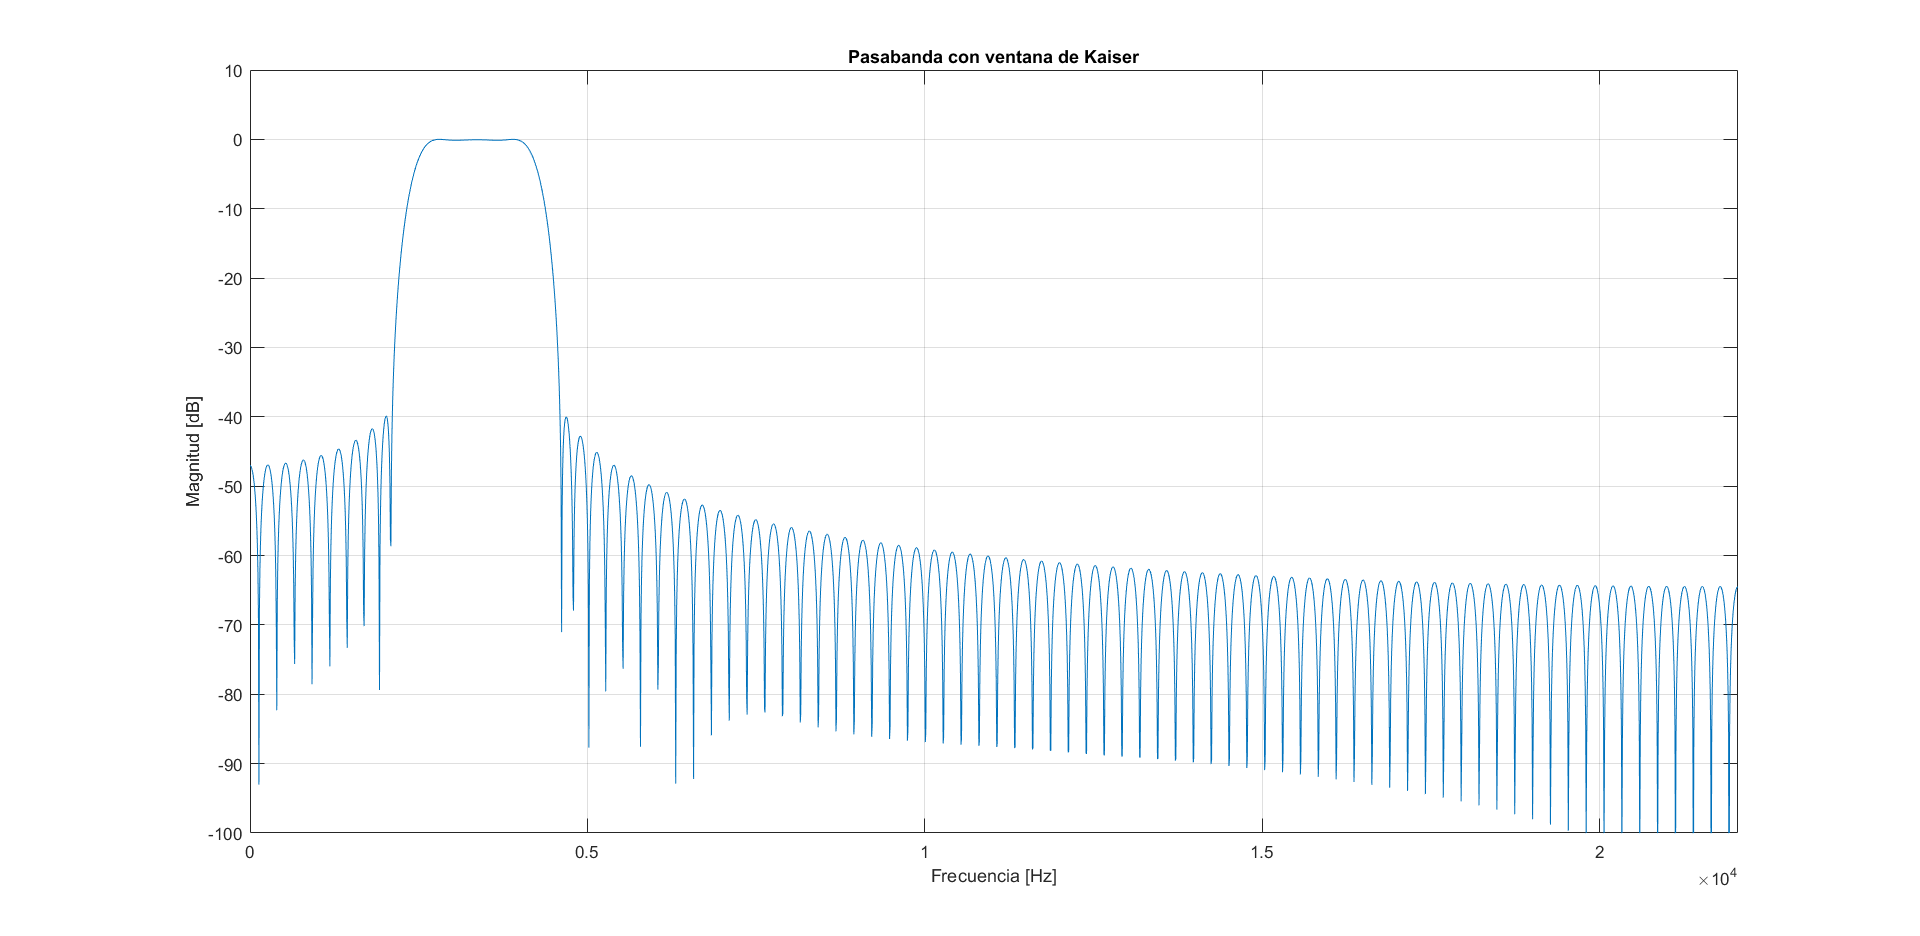
\includegraphics[scale=.35]{./images/2/modulo.png}
  \caption{Respuesta en frecuencia del pasabanda con ventana de Kaiser.}
\end{figure}
\begin{figure}[H]
  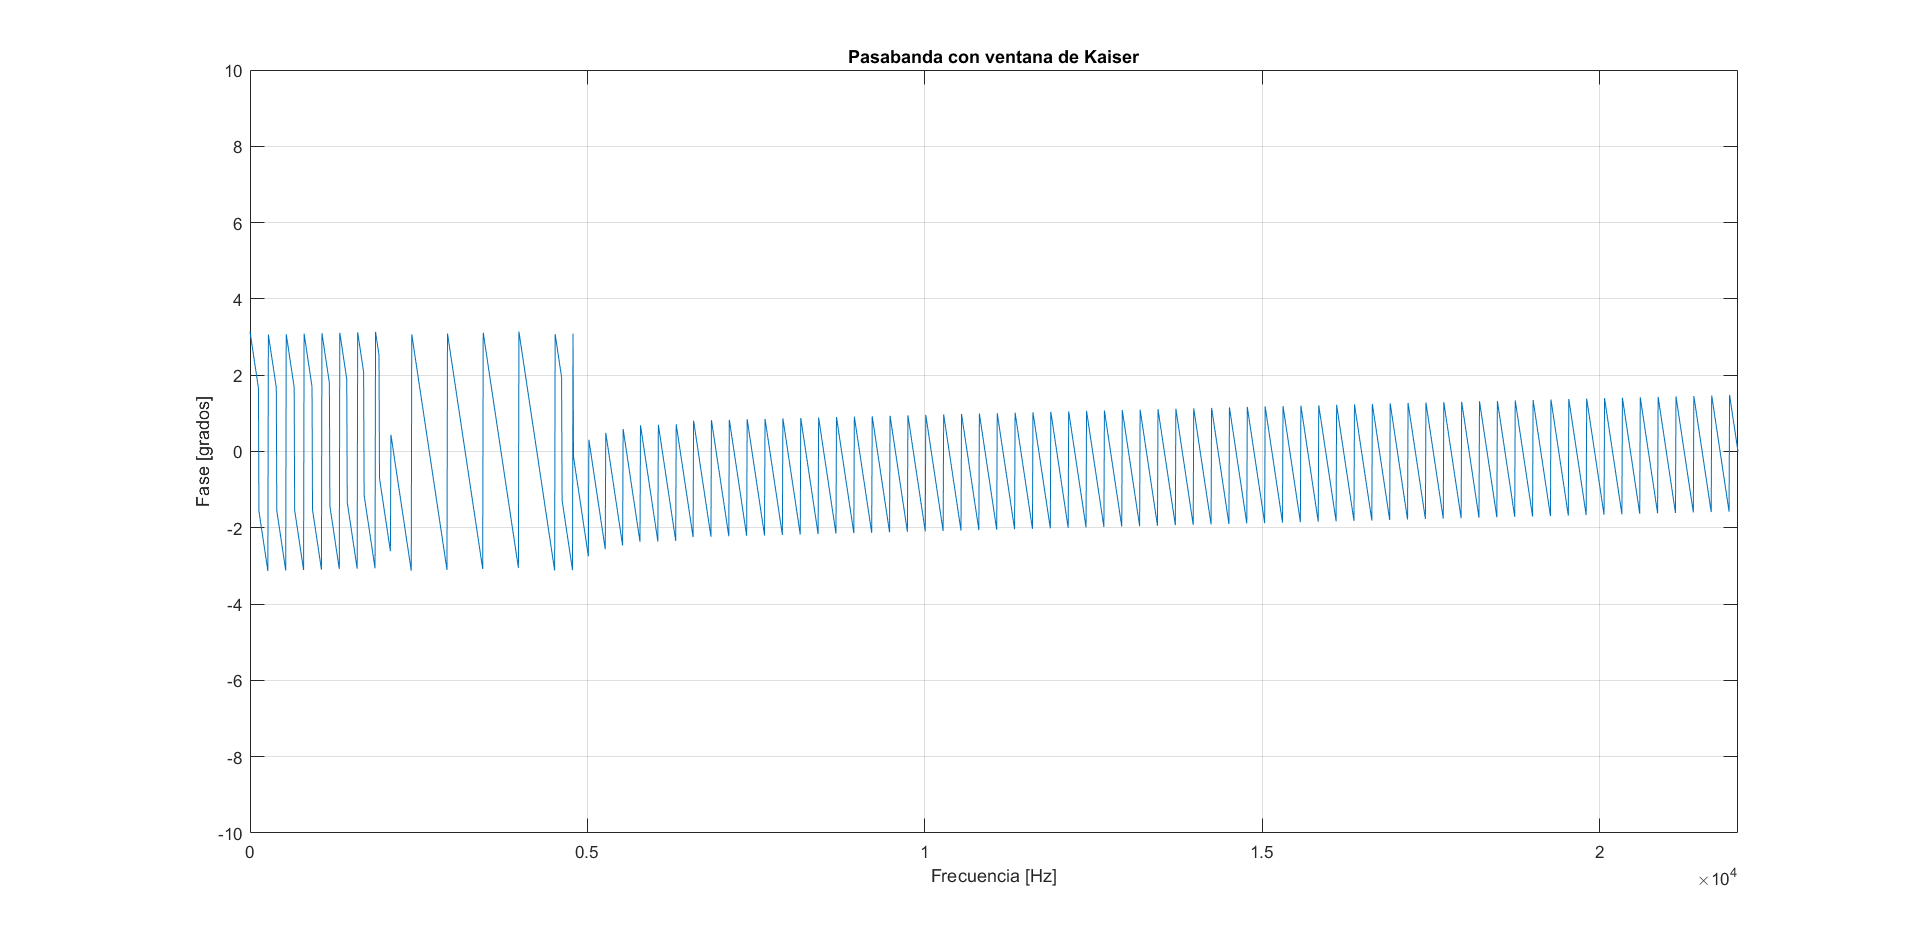
\includegraphics[scale=.35]{./images/2/fase.png}
  \caption{Fase del pasabanda con ventana de Kaiser.}
\end{figure}

Se puede observar que el filtro cumple plantilla de forma satisfactoria. Además se ve la máxima concentración de energía en el lóbulo principal, ya que los laterales se encuentran atenuados. Lo interesante de la aplicación de esta ventana es que se consigue un manejo muy detallado (a través del parámetro $\alpha$) de la relación entre el ancho del lóbulo principal y la amplitud de los laterales.
